\documentclass[]{article}

\usepackage{xcolor}
\usepackage{tikz}
\usepackage{pgfplots}

\newlength{\xdim}

\definecolor{calculate}{HTML}{D7191C}
\definecolor{copyBack}{HTML}{FDAE61}

%opening
\title{Multiprocessor Systems - Assignment I (MPI)}
\author{Adrian Holfter, Lucie Labadie}

\begin{document}

\maketitle

\section{Implementation}

\subsection{MPI-based Blocked Matrix-Matrix Multiplication}

\subsection{MPI-based LaPlace Approximation}

\section{Measurements}

\subsection{MPI-based Blocked Matrix-Matrix Multiplication}

The measurements were taken on the \emph{kraken.tek.bth.se} Server. The executables were compiled with the \texttt{-O3} option, to enable compiler optimizations. Every measurement was taken 10 times and the smallest value was used. Table \ref{tab:matrix-mult-runtime} shows the runtimes of the different versions.

\begin{figure}[h]
	\centering
	\begin{tabular}{|l|r|}
		\hline
		\textbf{Version} & \textbf{shortest runtime [s]} \\
		\hline
		Sequential single-threaded & 30.40 \\ 
		\hline 
		MPI 1 thread & 2.54 \\ 
		\hline 
		MPI 2 threads & 0.95 \\ 
		\hline 
		MPI 4 threads & 0.57 \\ 
		\hline 
		MPI 8 threads & 0.47 \\ 
		\hline 
	\end{tabular} 
	\caption{Runtime comparison for matrix multiplication}
	\label{tab:matrix-mult-runtime}
\end{figure}

Figure \ref{fig:maxtrix-mult-chart} shows the runtime breakdown for the MPI version per number of workers. It becomes clear that the percentage of time spent copying back the result matrix increases rapidly, which is because every worker sends back the \emph{whole} \texttt{C} matrix, even though only a small part of it actually contains work results.

\begin{figure}[h]
	\centering
	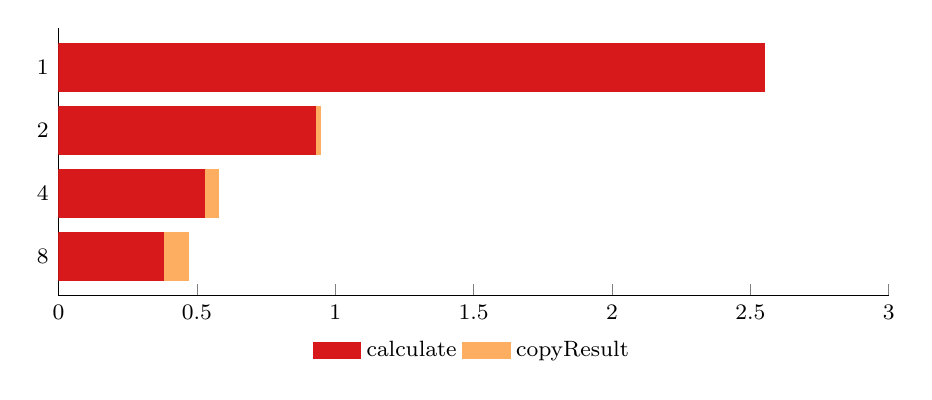
\begin{tikzpicture}
	\begin{axis}[
	xbar stacked,
	legend style={
		legend columns=4,
		at={(xticklabel cs:0.5)},
		anchor=north,
		draw=none
	},
	ytick=data,
	axis y line*=none,
	axis x line*=bottom,
	tick label style={font=\footnotesize},
	legend style={font=\footnotesize},
	label style={font=\footnotesize},
	xtick={0, 0.5, 1.0, 1.5, 2.0, 2.5, 3.0},
	width=1.0\textwidth,
	bar width=6mm,
	xlabel={Time in ms},
	yticklabels={1, 2, 4, 8},
	xmin=0,
	xmax=3.0,
	area legend,
	y=8mm,
	enlarge y limits={abs=0.625},
	]
	\addplot[calculate,fill=calculate] coordinates
	{(2.55,3) (0.927,2) (0.527,1) (0.380,0)};
	\addplot[copyBack,fill=copyBack] coordinates
	{(0.0,3) (0.02,2) (0.05,1) (0.09,0)};
	\legend{calculate, copyResult}
	\end{axis}  
	\end{tikzpicture}
	\caption{Runtime breakdown for matrix multiplication per number of workers}
	\label{fig:maxtrix-mult-chart}
\end{figure}

\subsection{MPI-based LaPlace Approximation}

\end{document}
